\documentclass[tikz,border=4pt]{standalone}
\usepackage[T1]{fontenc}
\usepackage[utf8]{inputenc}
\usepackage{amsmath,amssymb}
\usepackage{helvet}
\renewcommand{\familydefault}{\sfdefault}
\usepackage{pgfplots}
\pgfplotsset{compat=1.17}
\usetikzlibrary{arrows.meta,positioning,calc,fit,backgrounds,shapes.geometric}

\definecolor{cVis}{HTML}{1F77B4}
\definecolor{cTxt}{HTML}{D62728}
\definecolor{cProj}{HTML}{2CA02C}
\definecolor{cLLM}{HTML}{9467BD}
\definecolor{cConv}{HTML}{FF7F0E}
\definecolor{cAtt}{HTML}{17BECF}
\definecolor{cGray}{HTML}{7F7F7F}

\tikzset{
  blk/.style={draw, rounded corners=2pt, minimum height=8mm, align=center, font=\footnotesize, thick},
  tok/.style={draw, minimum size=3.2mm, inner sep=0pt},
  arr/.style={-{Stealth[length=2mm]}, thick},
}

\begin{document}
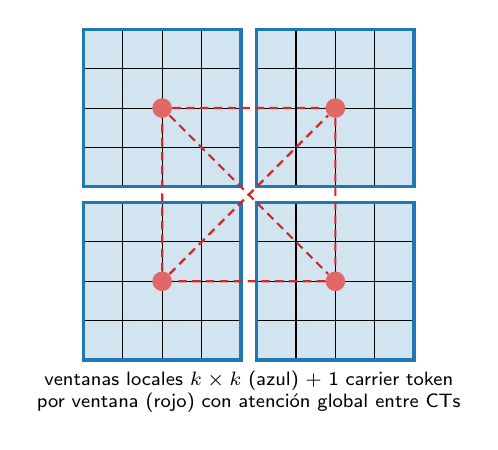
\begin{tikzpicture}[scale=.5]
  \foreach \wi in {0,1}{\foreach \wj in {0,1}{
    \pgfmathsetmacro{\ox}{\wi*4.4}\pgfmathsetmacro{\oy}{\wj*4.4}
    \foreach \i in {0,...,3}{\foreach \j in {0,...,3}{\draw[fill=cVis!20] (\ox+\i,\oy+\j) rectangle ++(1,1);}}
    \draw[very thick, cVis] (\ox,\oy) rectangle ++(4,4);
    \node[circle, fill=cTxt!70, inner sep=2.5pt] (c\wi\wj) at (\ox+2,\oy+2) {};}}
  \draw[cTxt, thick, densely dashed] (c00) -- (c01) -- (c11) -- (c10) -- (c00) -- (c11); \draw[cTxt, thick, densely dashed] (c01) -- (c10);
  \node[font=\scriptsize, align=center] at (4.2,-0.8) {ventanas locales $k\times k$ (azul) + 1 carrier token\\por ventana (rojo) con atención global entre CTs};
\end{tikzpicture}
\end{document}
